\section{Overview of Three Deployments}

\begin{figure}[t]
\begin{center}
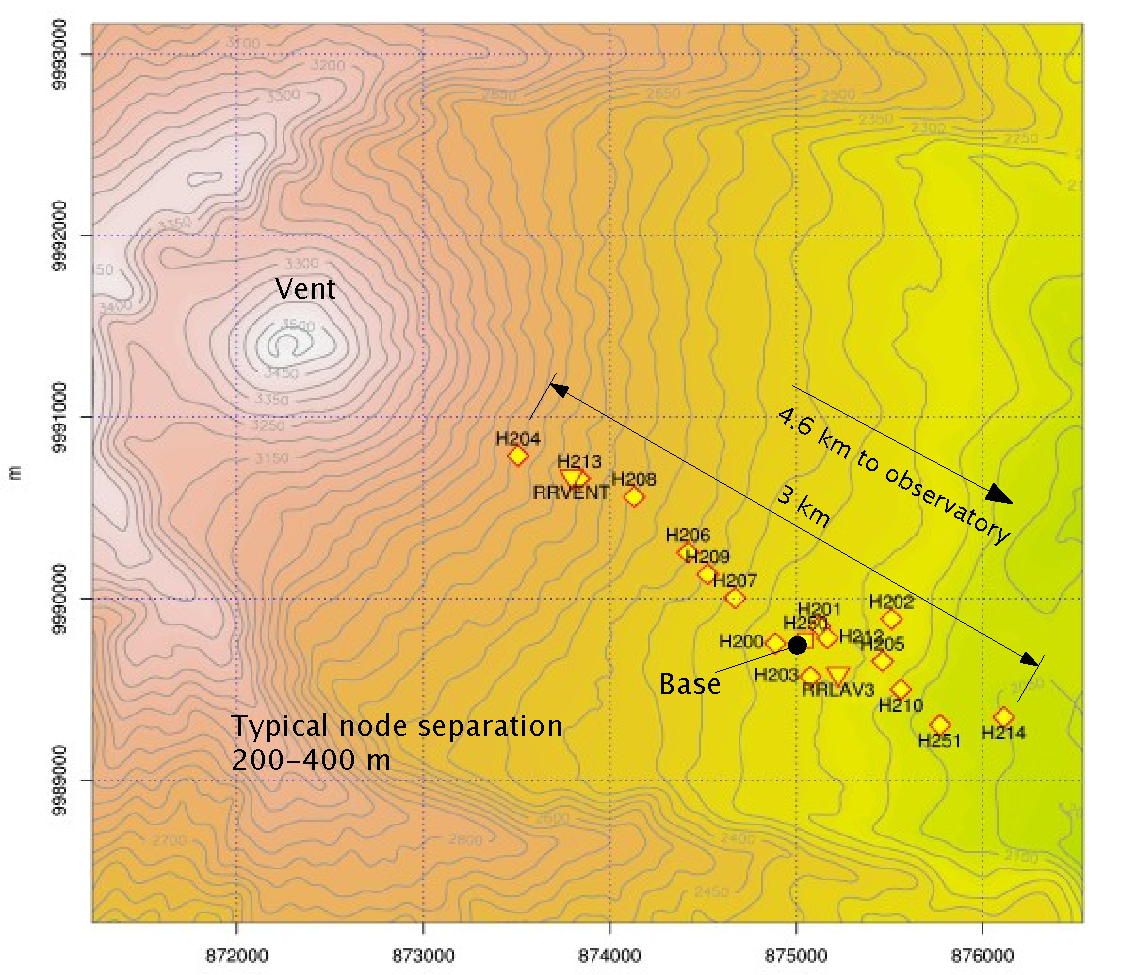
\includegraphics[width=0.8\hsize]{./3-evaluation/figs/2005-deployment-map.pdf}
\end{center}
\caption{\textbf{2005 deployment location.} The figure shows the location of
our second volcano deployment in 2005: 16 nodes deployed on Reventador
Volcano.}
\label{introduction-fig-deployment-map-2005}
\end{figure}

In total, we have performed three deployments of iterations of our system at
active volcanoes in Ecuador. Figs.~\ref{introduction-fig-deployment-map-2005}
and \ref{introduction-fig-deployment-map-2007} show the location and layout
of the second and third deployment. All three are summarized below:

\begin{figure}[t]
\begin{center}
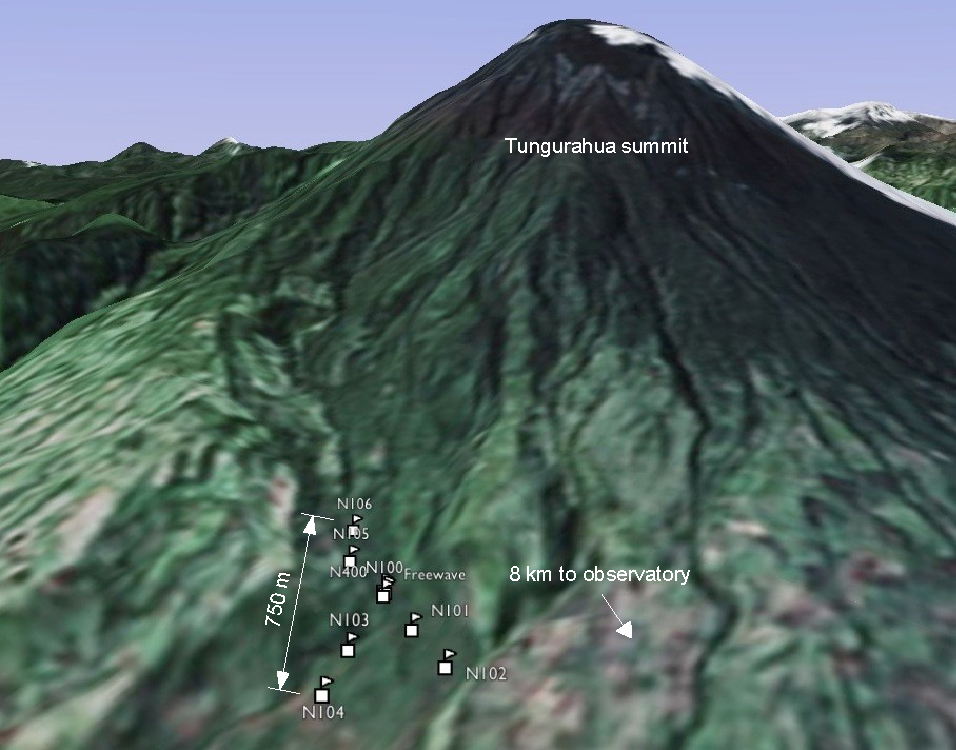
\includegraphics[width=0.8\hsize]{./3-evaluation/figs/2007-deployment-map.pdf}
\end{center}
\caption{\textbf{2007 deployment location.} The figure shows the locations of
our third volcano deployment in 2007: eight nodes deployed on Tungurahua
Volcano.}
\label{introduction-fig-deployment-map-2007}
\end{figure}

\begin{enumerate}

\item \textbf{July, 2004, Tungurahua Volcano:} We deployed three infrasonic
monitoring nodes continuously transmitting at 102~Hz to a central aggregator
node, which relayed the data over a wireless link to the observatory
approximately 9~km away.  Our network was active from July 20--22, 2004, and
collected over 54~hours of infrasonic signals.

\item \textbf{August, 2005, Reventador Volcano:} This deployment featured a larger,
more capable network consisting of sixteen nodes fitted with seismoacoustic
sensors deployed in a 3~km linear array.  Collected data was routed over a
multi-hop network and over a long-distance radio link to a logging laptop
located at the observatory 9~km away from deployment site.  Over three weeks
the network captured 230 volcanic events.

\item \textbf{July, 2007, Tungurahua Volcano:} We returned to Tungurahua Volcano in
2007 and deployed eight sensor nodes in order to test Lance, a framework for
optimizing high-resolution signal collection. The network was operational for
a total of 71~hours, during which time we downloaded 77~MB of raw data.

\end{enumerate}

\section{Deploying on Volc\'{a}n Reventador}

Volc\'{a}n Reventador is located in northern Ecuador, a three hour drive from
the capital, Quito.  Long dormant, Reventador reawakened suddenly in 2002,
erupting with massive force.  Ash thrown into the air blanketed the streets
of Quito 100~km to the east, closing schools and the airport.  Pyroclastic
flows raced down the mountain flattening forests, displacing an oil pipeline,
and severing a major highway.  After 18 months of quiescence, renewed
activity began in November 2004.  During our deployment, Reventador's
activity was characterized by discrete, relatively small explosive events,
ejecting incandescent blocks, gas, and ash several times a day.
Corresponding seismic activity was manifested by explosion earthquakes,
extended-duration shaking (tremor), and shallow rock fracturing earthquakes
that may have been associated with magma migration within the volcano.

Several features of Volc\'{a}n Reventador made it ideal for our
experiment.  Reaching 3,500~meters at its peak, Reventador sits at a
low elevation compared to other Ecuadorean volcanoes making deployment
less strenuous.  Its climate is moderate with temperatures ranging
between 10 and 30 degrees Celsius.  Pyroclastic flows produced by the
large explosion in 2002 left large parts of the flanks denuded of
vegetation.  With the effectiveness of our radio antennas severely
degraded by obstacles to line-of-sight, the lack of vegetation
simplified sensor node positioning.

Our base while working at Reventador was the Hosteria El Reventador, a small
hotel located nearby on the highway from Quito to Lago Agria.  The hotel
provided us with space to set up our equipment and ran an electric generator
to power our laptops and other equipment at the makeshift observatory.

\subsection{Network Hardware}

Our network consisted of 16~stations equipped with seismic and acoustic
sensors.  Each station consisted of a Moteiv TMote Sky~\cite{moteiv} wireless
sensor network node, an 8~dBi~2.4GHz external omnidirectional antenna,
seismometer, microphone, and a custom hardware interface board.
Fourteen~nodes were fitted with a Geospace Industrial GS-11 geophone, a
single-axis seismometer with a corner frequency of 4.5~Hz, oriented in the
vertical plane of motion.  The remaining two~nodes were equipped with
triaxial Geospace Industries GS-1 seismometers with corner frequencies of
1~Hz, yielding separate signals in each of the three axes.

The TMote Sky is a descendant of the UC Berkeley Mica ``mote'' sensor node.
It features a Texas Instruments MSP430 microcontroller, 48~KB of program
memory, 10~KB of SRAM, 1~MByte of external flash memory and a 2.4GHz Chipcon
CC2420 IEEE 802.11.4 radio.  The TMote Sky was designed to run
TinyOS~\cite{tinyos-asplos00}, and all of our software development made use
of this environment.  We chose the TMote Sky for several reasons.  The MSP430
microprocessor provides a large number of configurable ports, easily
supporting external devices.  The large amount of flash memory was useful for
buffering collected data, as described below.

We built a custom hardware board to integrate the TMote Sky with the
seismoacoustic sensors.  The board features up to four Texas Instruments
AD7710 analog to digital converters (ADCs) providing up to 24~bits per
channel of resolution.  Although the MSP430 microcontroller provides on-board
ADCs, they are unsuitable for our application.  First, they provide only
16~bits of resolution while we required at least 20~bits.  Second,
seismoacoustic signals require an aggressive filter centered around 50~Hz.
Due to the infeasibility of implementing such a filter using analog
components, it is usually approximated digitally, requiring several factors
of oversampling.  To perform this filtering, the AD7710 is sampling at over
30~kHz while presenting an output word rate of 100~Hz.  The high sample rate
and computation required by digital filtering are best delegated to a
specialized device.

Each sensor node was powered by a pair of alkaline D~cell batteries.  The
remote location of our network made it important to choose batteries
maximizing node lifetime.  D~cells provided the best combination of low cost
and high capacity, and are able to power a node for over a week.
Approximately 75\% of the power drawn by each node is consumed by the sensor
interface board, primarily due to the high power consumption of the ADCs.
During our three week deployment we swapped batteries between 4~and~5 times.
This was more often than strictly necessary, but battery changes were often
performed while visiting nodes for other reasons.

\subsection{Sensor Network Device Enclosures and Physical Setup}

\begin{figure}[t]
\label{architecture-fig-picture}
\begin{center}
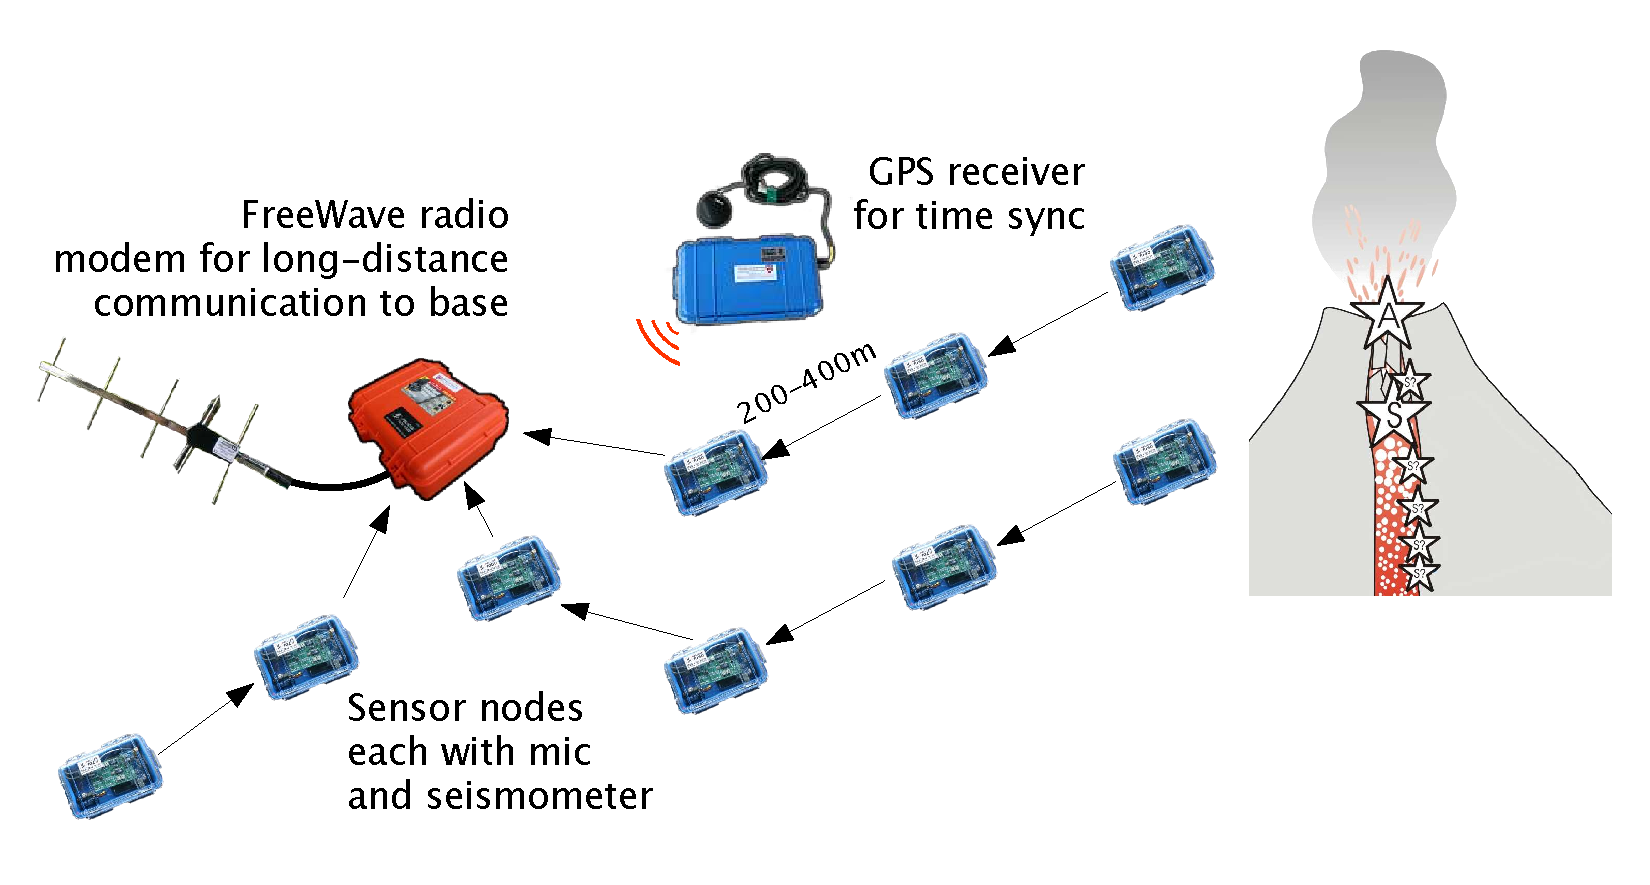
\includegraphics[width=0.7\hsize]{./3-evaluation/figs/schematic}
\end{center}
\caption{\textbf{Schematic representation of our sensor network
architecture.}}
\end{figure}

A single sensor network node, interface board, and battery holder were all
housed inside a small weatherproof and watertight Pelican case.  We installed
environmental connectors through the case allowing cables to external sensors
and antennae to be attached without opening the case and disturbing the
equipment inside.  When working in wet and gritty conditions these became a
tremendous asset.

\begin{figure}[t]
\begin{center}
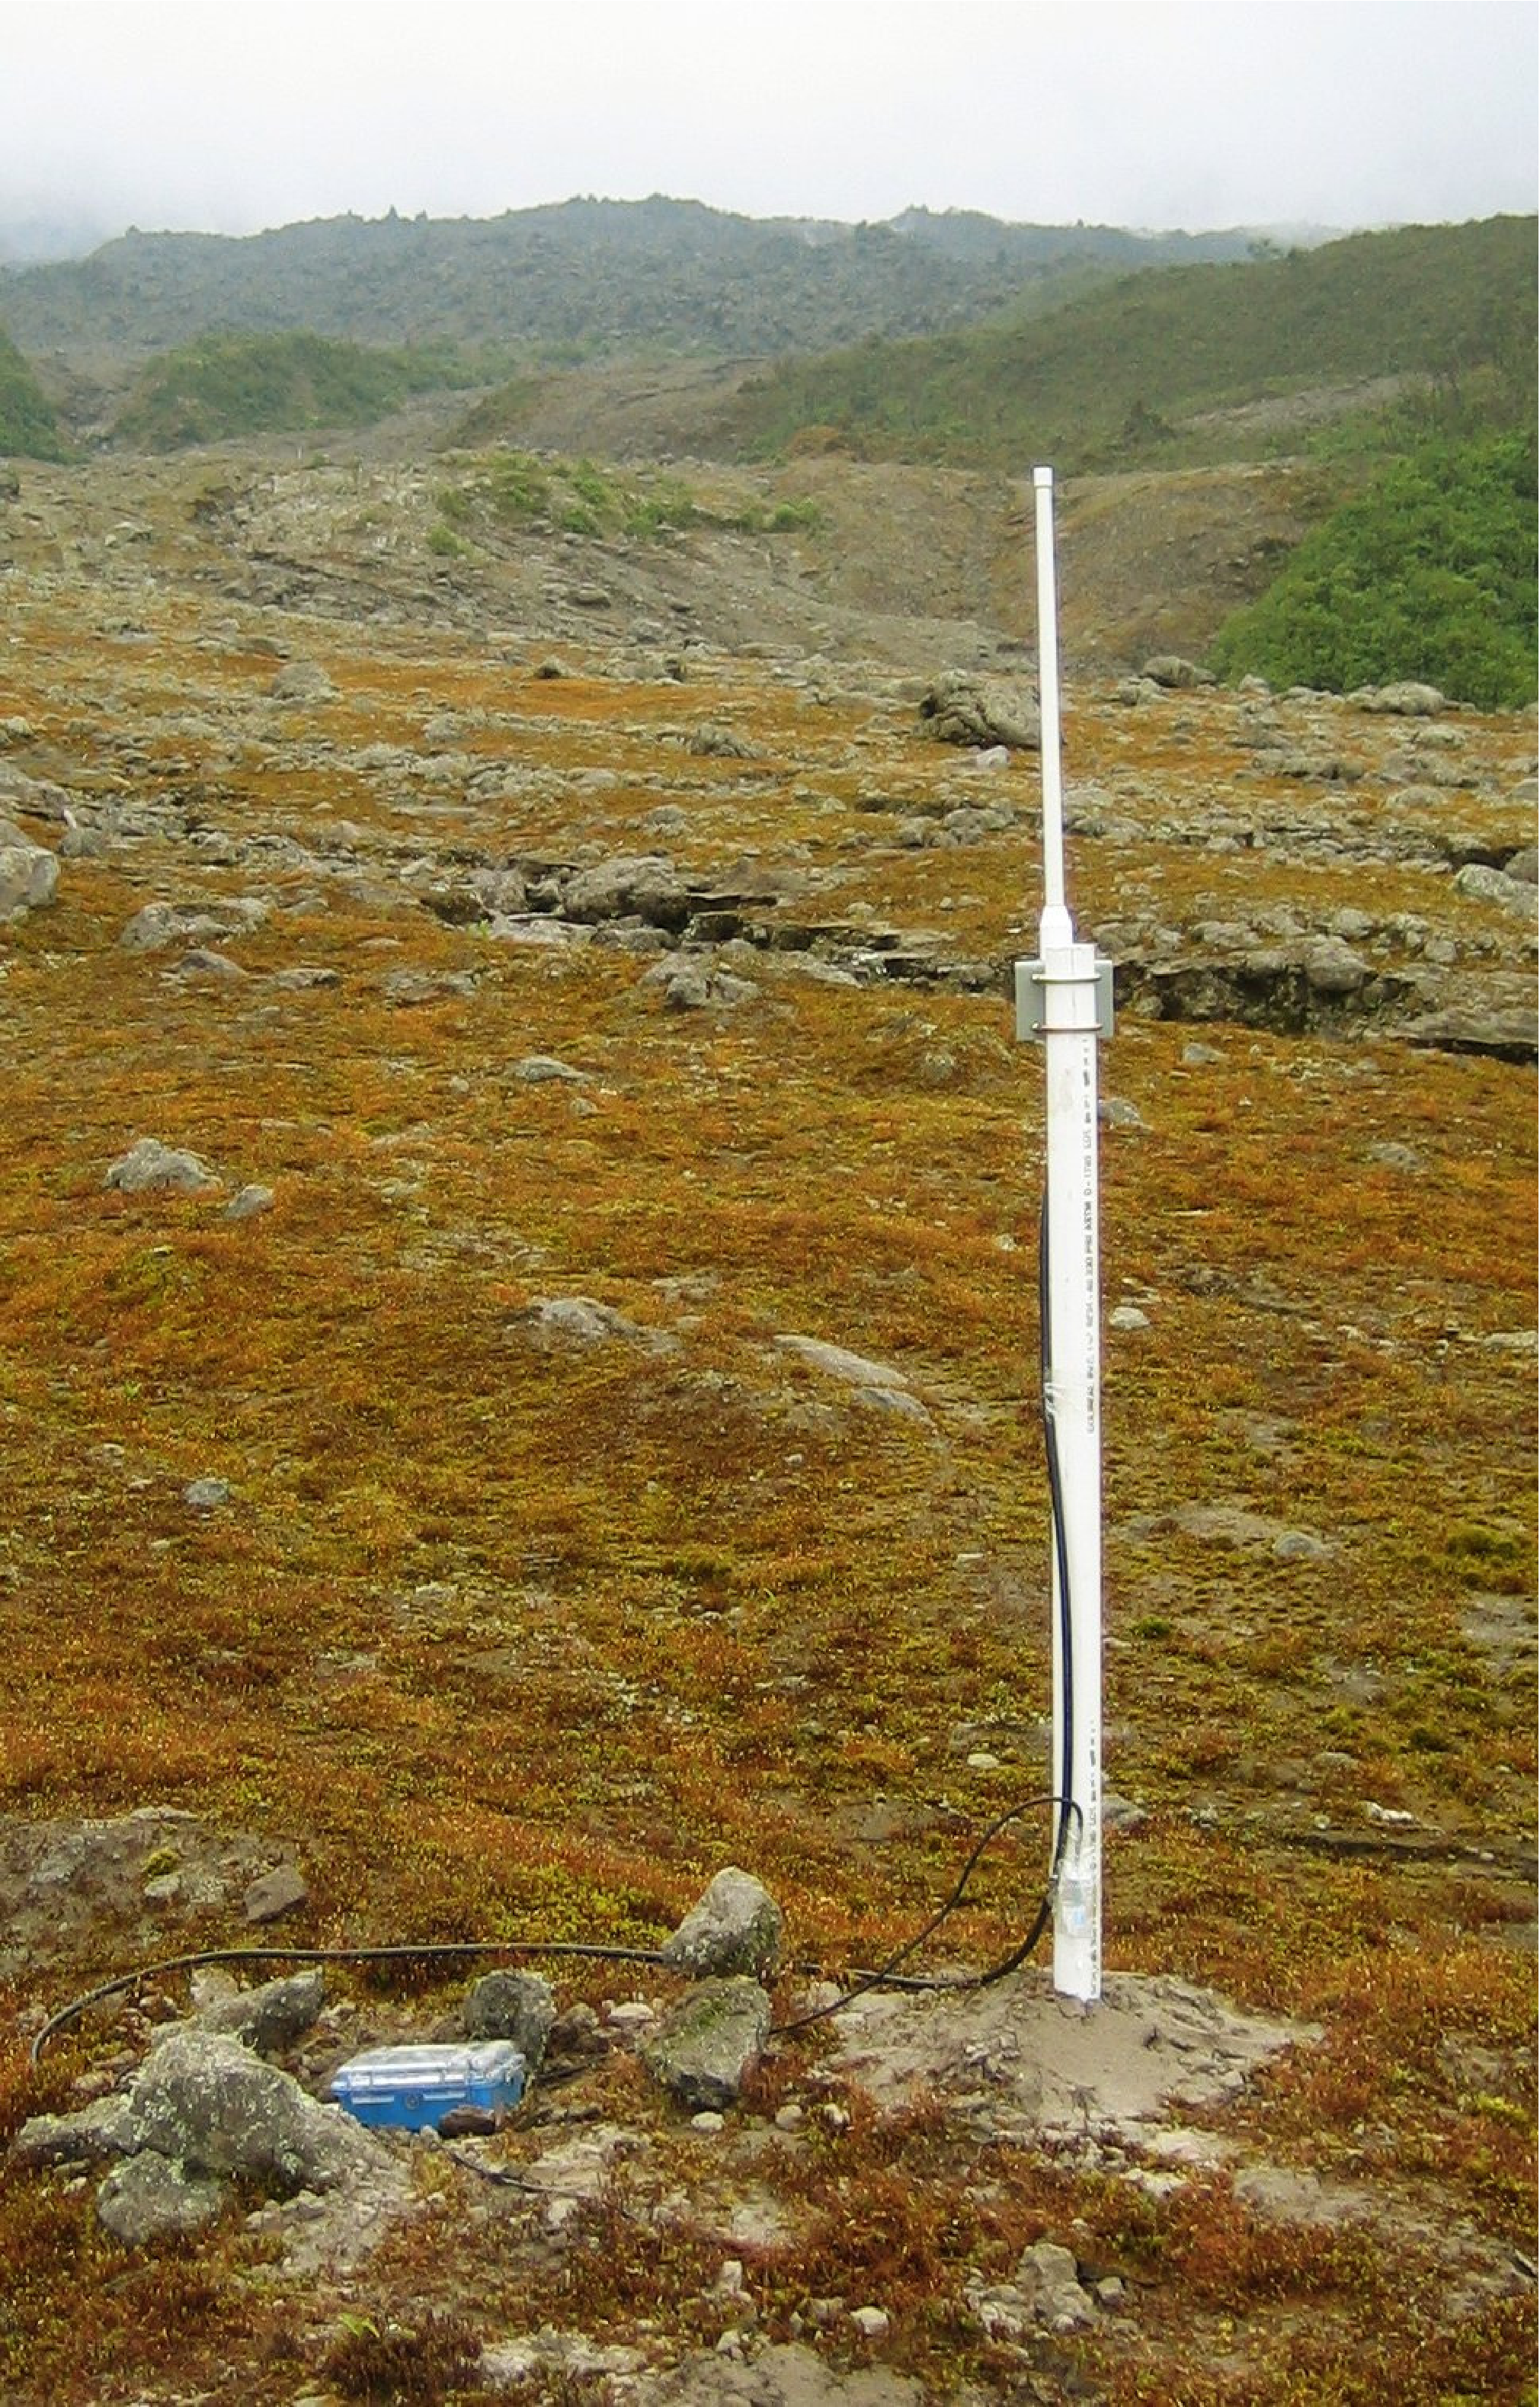
\includegraphics[width=0.7\hsize]{./3-evaluation/figs/Station}
\end{center}
\caption{\textbf{One of our two-component stations.  The blue Pelican
Case contains the wireless sensor network node and hardware interface board.
The external antenna is mounted on the PVC pole to reduce ground effects.
A microphone is taped to the PVC pole and a single seismometer is buried
nearby.}}
\label{fig-station}
\end{figure}

Installing a station involved covering the Pelican case with rocks to anchor
it and shield the contents from direct sunlight.  Cables were run from the
box to each sensor and to the antenna.  The antenna was elevated on a 1.5~m
length of PVC piping to reduce ground effects which reduce radio range.  The
seismometers were buried nearby, but far enough away to remain undisturbed by
any wind-induced shaking of the antenna pole.  The microphone was usually
mounted on the antenna pole and shielded from the wind and elements with
plastic tape.  Installation took a matter of minutes and the equipment was
sufficiently light and small that six stations could be carried in a large
pack.  The PVC poles were light but bulky and proved the most awkward part of
each station to cart around.

\subsection{Network Location and Topology}

We installed our stations in a roughly linear configuration, radiating away
from the vent and producing an aperture of over 3~km.  We attempted to
position the stations as far apart as the radios on each node would allow.
Although our antennas could maintain radio links of over 400~m, the geography
at the deployment site occasionally required installing additional stations
to maintain radio connectivity.  Other times we would deploy a node expecting
it to communicate with an immediate neighbor but later notice that that node
was bypassing its closest companion in favor of a node closer to the base
station.  Most nodes communicated with the base station over three or fewer
hops, but a few were moving data over as many as six.

In addition to the sensor nodes, several other pieces of equipment
were used.  Three Freewave~\cite{freewave} radio modems provided a
long-distance, reliable radio link between the sensor network and the
observatory laptop.  Freewave modems at the deployment site and the
observatory used a 9~dBi directional Yagi antenna to relay data via a
repeater station, installed on a hill with good line-of-sight to both
endpoints.  Each Freewave required a car battery for power, recharged
by solar panels.  A small number of Crossbow~\cite{xbow} MicaZ sensor
network nodes served in supporting roles.  One interfaced between the
network and the Freewave modem; another was attached to a GPS receiver
to provide a global timebase.

\begin{figure}[t]
\label{includegraphics-fig-plot}
\begin{center}
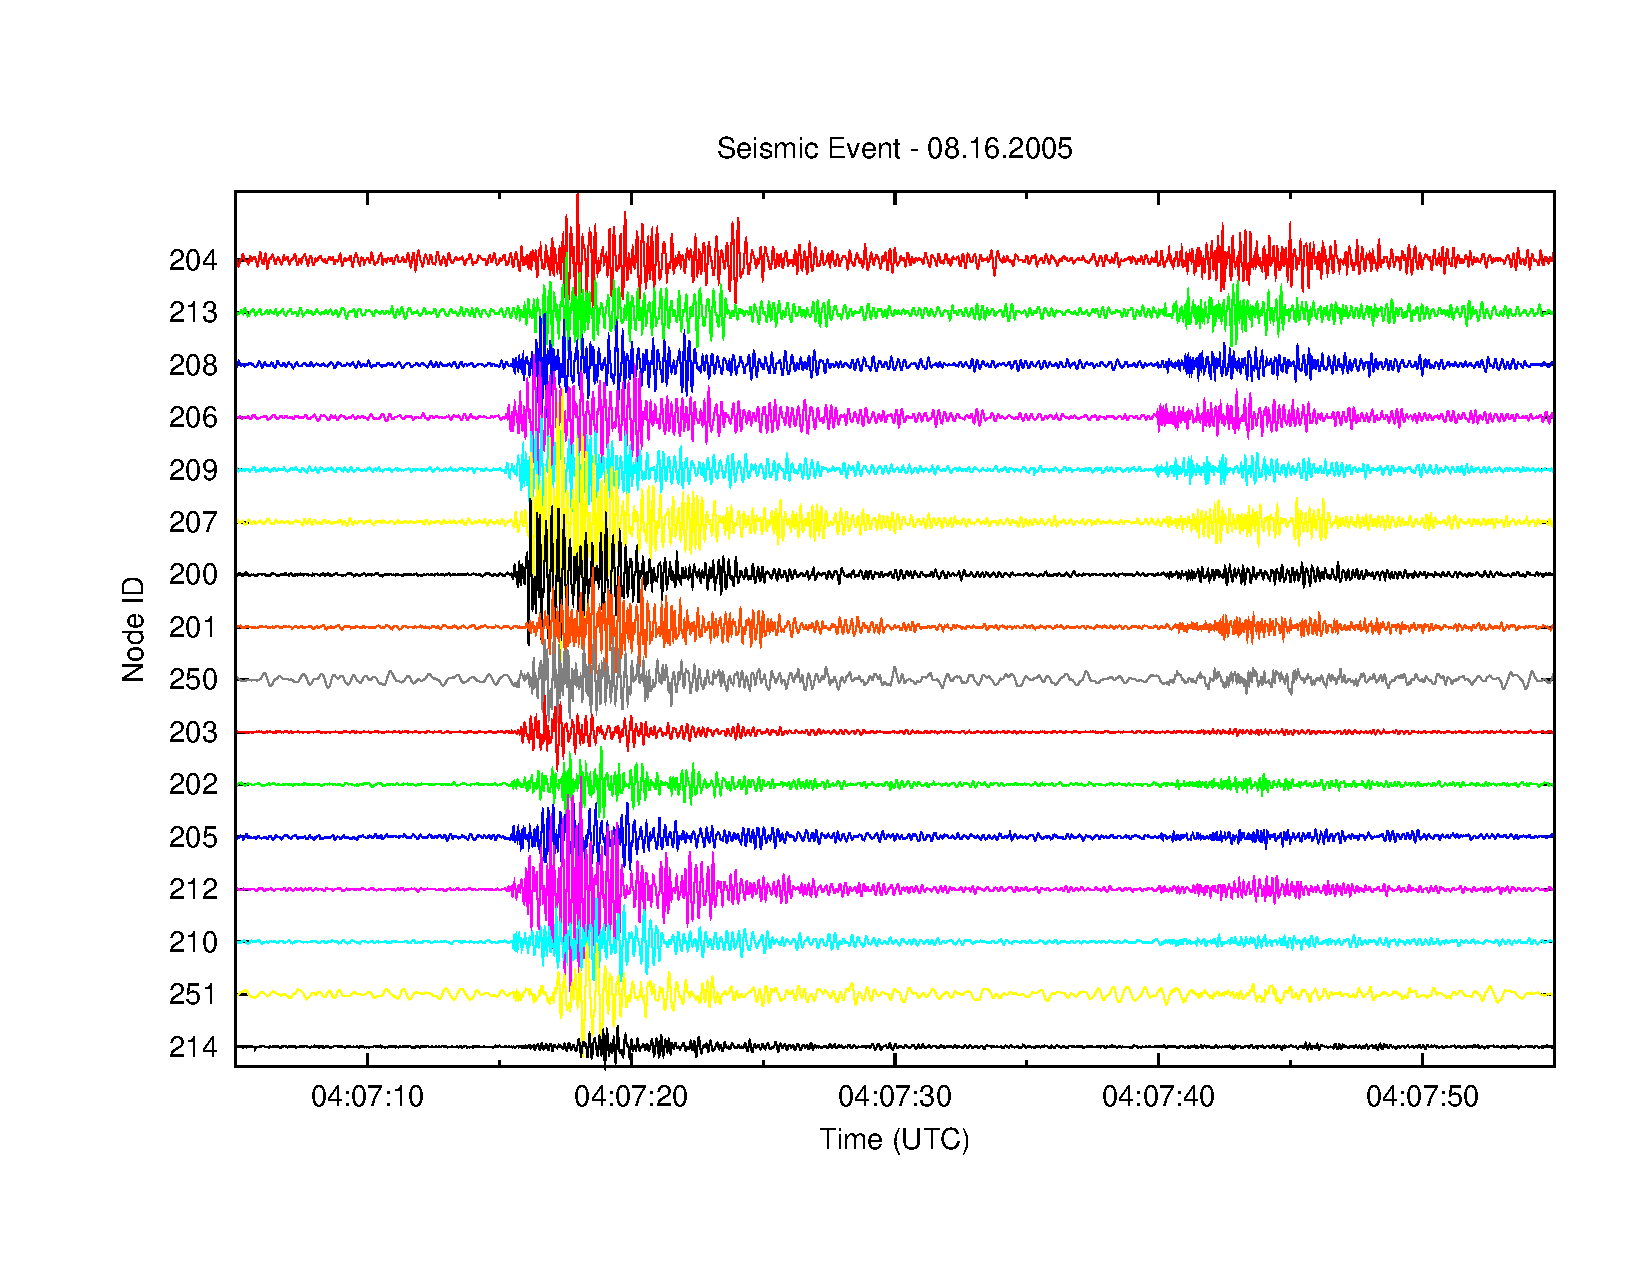
\includegraphics[width=0.7\hsize]{./3-evaluation/figs/TEST}
\end{center}
\caption{\textbf{Example of an event captured by our network.}  Only
seismic signals are shown.  The event shown was a Volcano Tectonic (VT) event
and had no interesting acoustic component.  Data shown has undergone several
rounds of post-processing including mapping to GMT time.}
\end{figure}

\begin{figure}[t]
\begin{center}
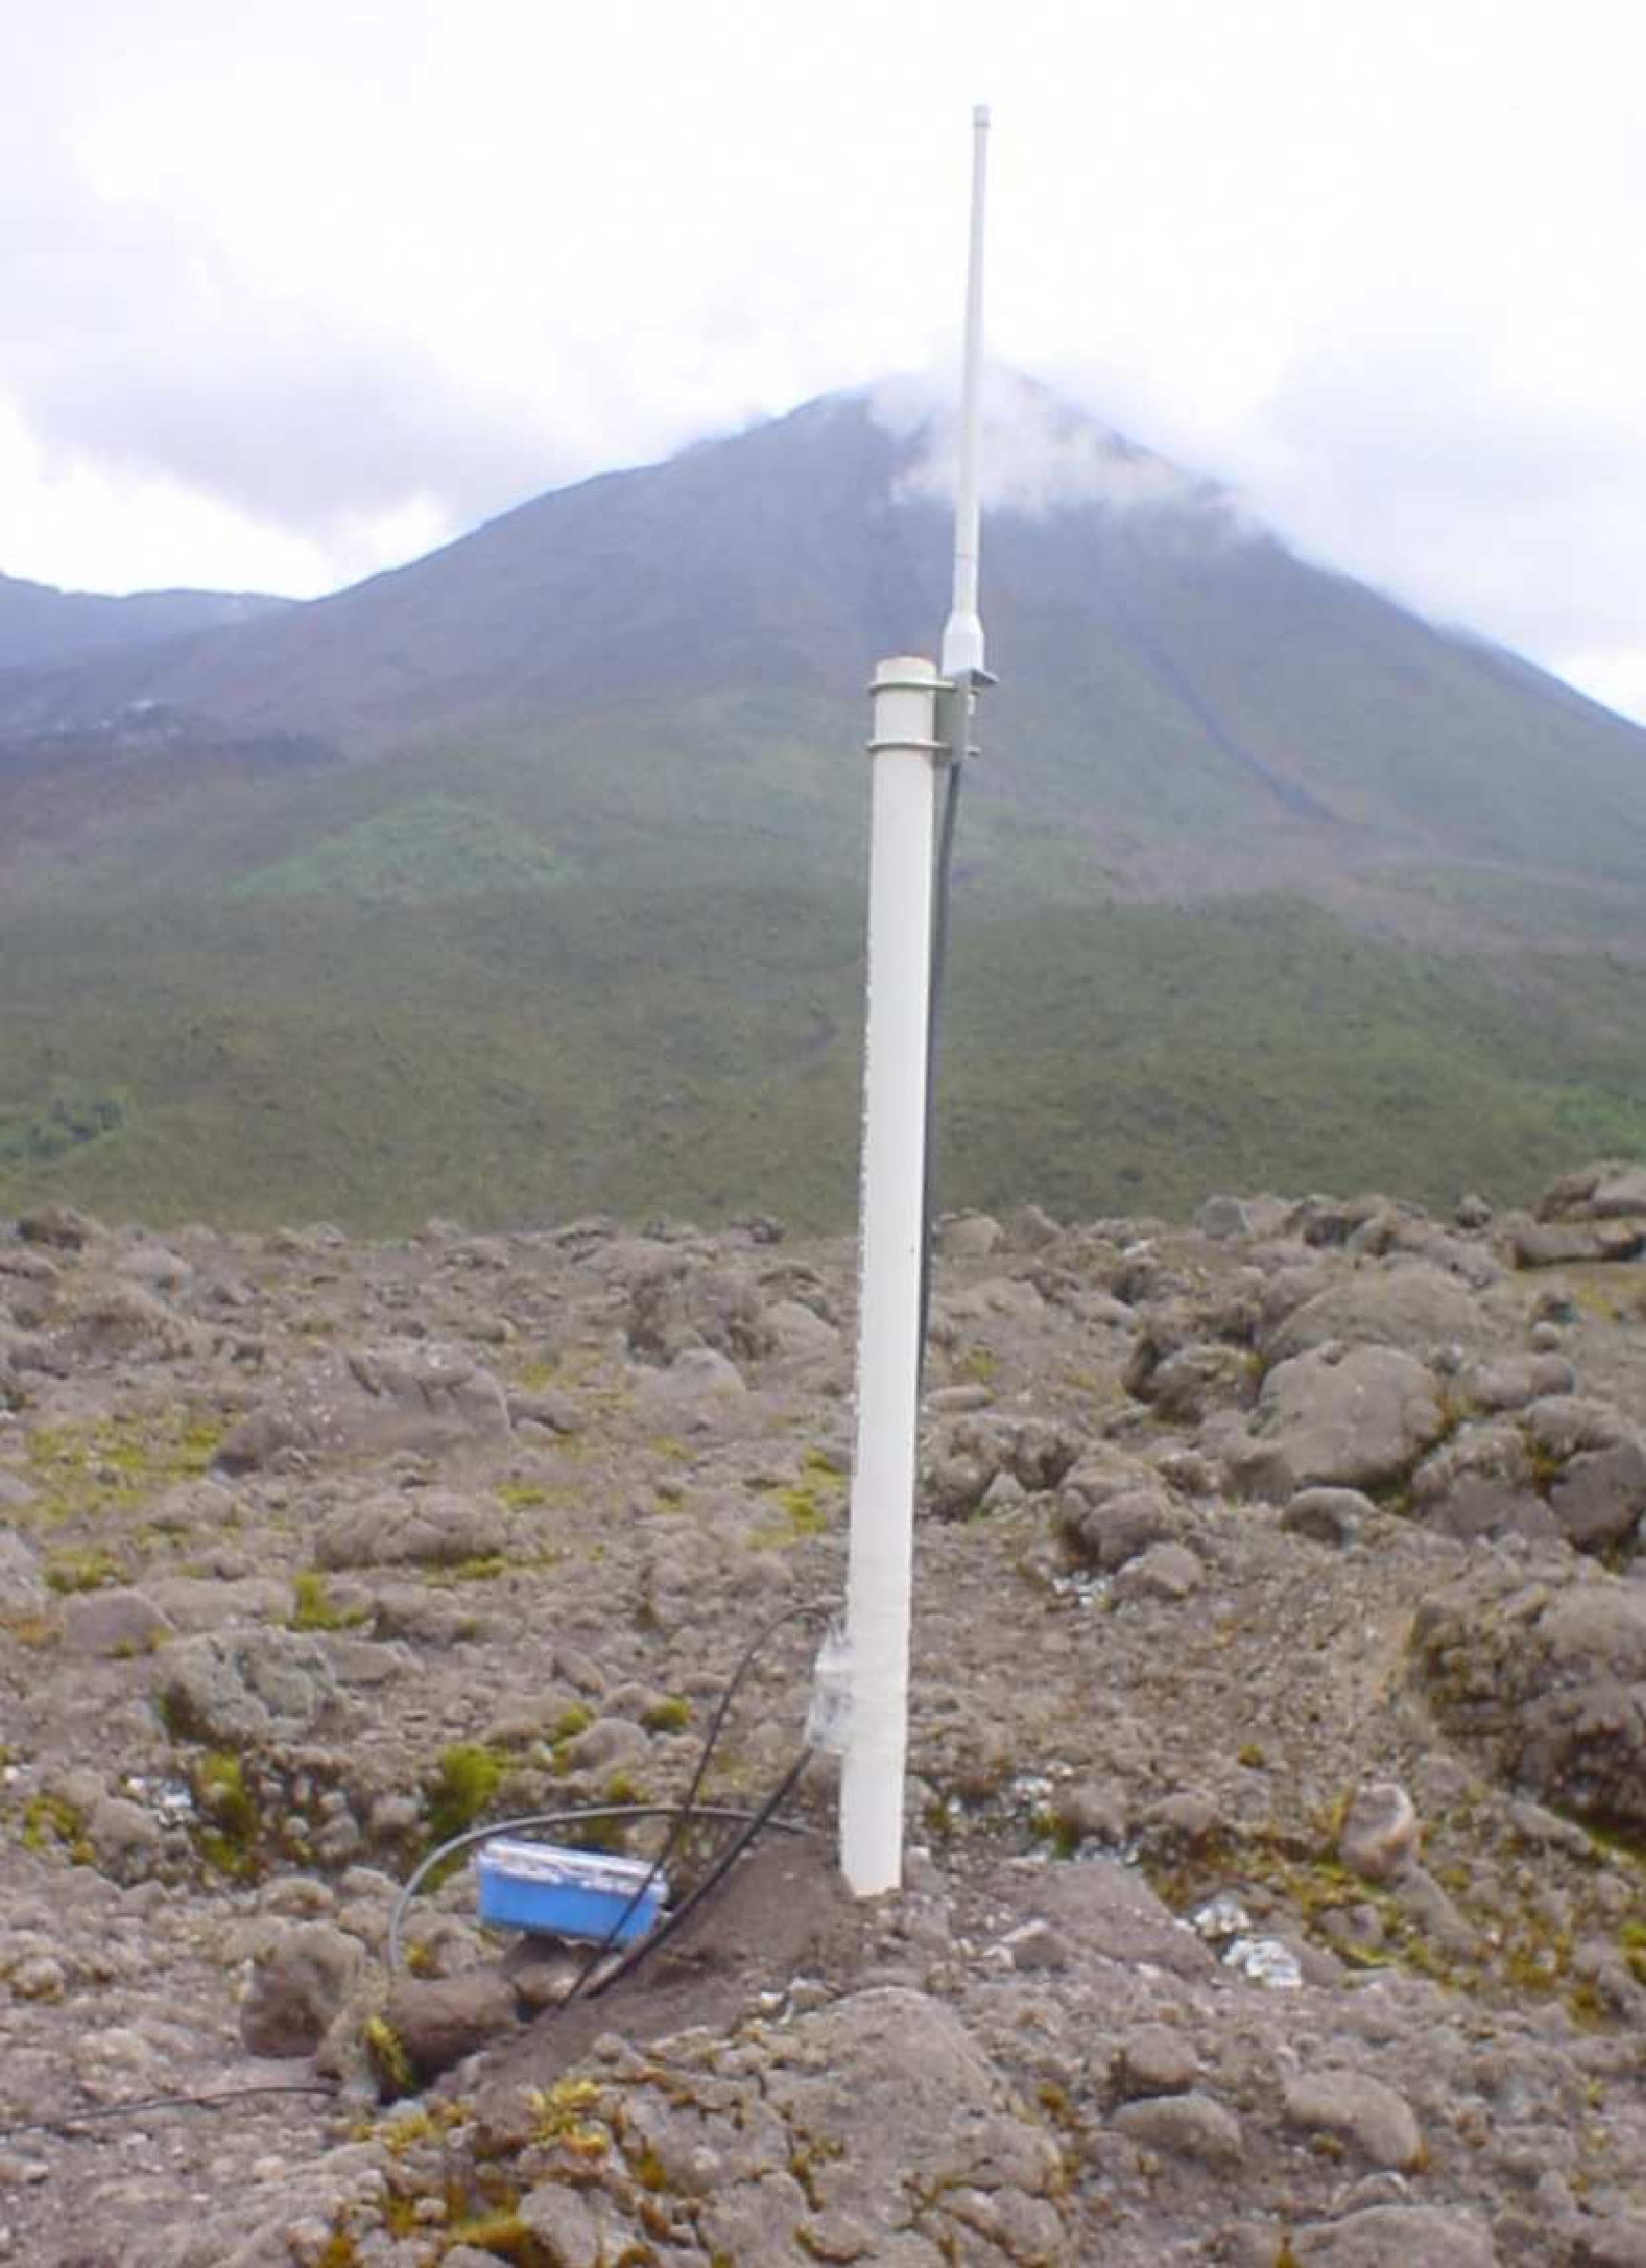
\includegraphics[width=0.7\hsize]{./3-evaluation/figs/Node-212-5}
\end{center}
\caption{\textbf{One of our two-component stations.} The blue Pelican
Case contains the wireless sensor network node and hardware interface board.
The external antenna is mounted on the PVC pole to reduce ground effects.
A microphone is taped to the PVC pole and a single seismometer is buried
nearby.}
\label{includegraphics-fig-station2}
\end{figure}

\XXXnote{GWA: Pulled from OSDI'06 design.}

\subsection{Sensor hardware}
\label{evaluation-sec-hardware}

\begin{figure}[t]
\label{evaluation-fig-station}
\begin{center}
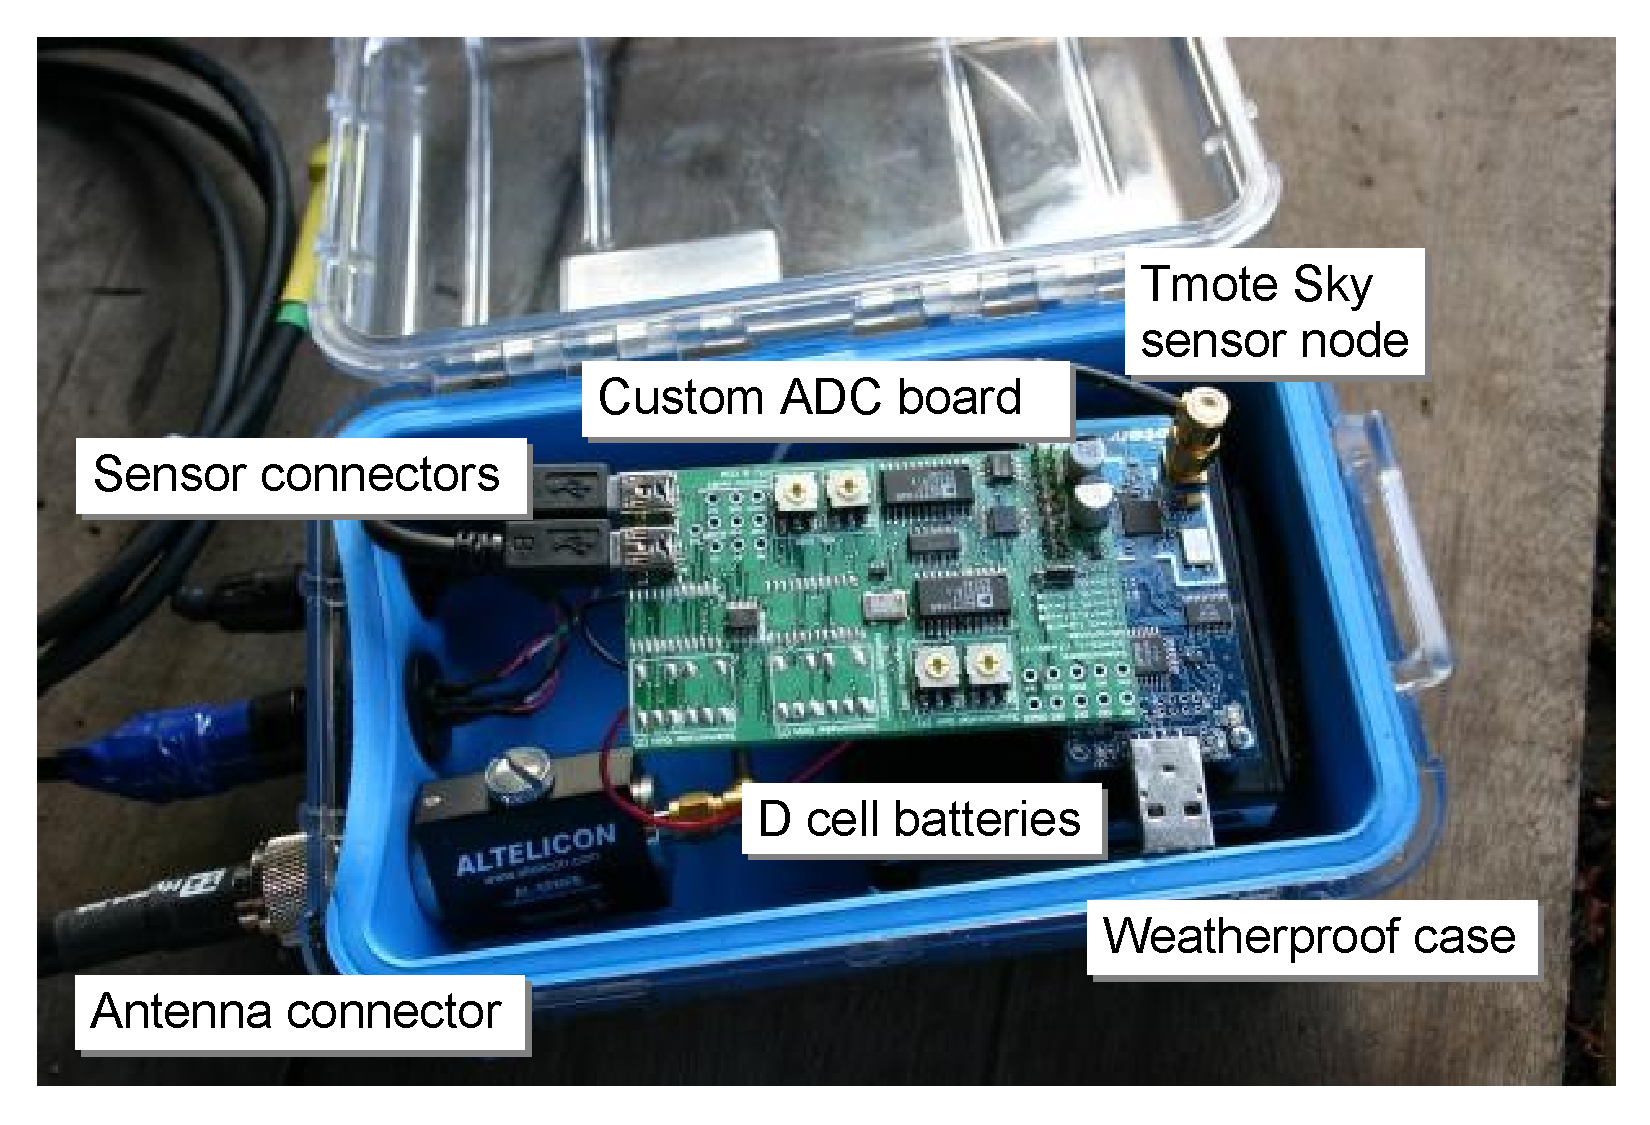
\includegraphics[width=1.0\hsize]{./3-evaluation/figs/Station2-small.pdf}
\end{center}
\caption{\textbf{Our wireless volcano monitoring sensor node.}}
\end{figure}

%We deployed 16 wireless monitoring stations onto Volc\'{a}n Reventador.
%Nodes were arranged in a roughly-linear configuration radiating from the vent
%and spanning over 3km.  Figure REFERENCE shows the locations of each node as
%well as those of several wired monitoring stations deployed nearby.
%\GWAnote{Do we event want to include this figure again? It takes up a lot of
%space but it probably would be nice to have...}

Our wireless sensor node (Figure~\ref{evaluation-fig-station}) is based on
the TMote Sky~\cite{moteiv} platform, which integrates a TI~MSP430 processor,
10~KB of SRAM, 48~KB of program ROM, 1~MByte of flash memory, and a Chipcon
CC2420 radio. All software is implemented in TinyOS~\cite{tinyos-asplos00}.
We designed a custom sampling board that provides four channels of 24-bit
analog-to-digital conversion (TI~AD7710). 
%While the MSP430 provides several channels of ADC, its resolution of 16~bits
%was inadequate for our needs.

Nodes were interfaced to either a single-axis seismometer (GeoSpace GS-11) or
three seismometers in a triaxial configuration (GeoSpace GS-1). 
%The GS-11 sensors are inexpensive and lightweight, but are only sensitive at
%frequencies above 4.5~Hz. In contrast, the GS-1 sensors have a corner
%frequency of 1~Hz but are significantly more expensive and heavy. 
Both sensors are passive instruments; ground motion generates a voltage which
is amplified and digitized by the sampling board.  In addition, each node was
attached to an omnidirectional microphone (Panasonic WM-034BY). This
microphone has been used in other infrasonic monitoring
studies~\cite{johnson-etal-04b}.

% MDW: Node 204 talked to 206 which was 1055 meters away!
Each node was equipped with an 8.5~dBi omnidirectional antenna mounted on
1.5~m of PVC pipe.  This permitted line-of-sight radio range of over 1~km
without amplification; nodes were typically placed 200-400~m apart in our
deployment. Nodes were powered by two D-cell batteries with a lifetime of
approximately 1~week.  Each node was enclosed in a weatherproof Pelican case.

Several other pieces of hardware complete the system. FreeWave radio modems
provided a long-distance radio link between the sensor array and the volcano
observatory, 4.6~km away. A laptop located at the observatory logged data and
was used to monitor and control the network.  Finally, to establish a global
timebase, we used a single Crossbow MicaZ~\cite{xbow} mote interfaced to a
GPS receiver (Garmin OEM~18~LVC).  The GPS receiver provided a 1~Hz pulse
that is accurate to GPS time within 1~$\mu$s, and acted as the root of the
network time synchronization protocol.
%as described in Section~\ref{evaluation-sec-timing}.

\subsection{Network topology and status monitoring}

Nodes form a multihop routing tree rooted at the gateway node that is
physically attached to the FreeWave modem; we use a variant of
MintRoute~\cite{awoo-multihop} that uses the CC2420's Link Quality Indicator
metric to select routing paths. Each node transmits a {\em status message}
every 10~sec that includes its position in the routing tree, buffer status,
local and global timestamps, battery voltage, and other information. 
%These status messages form the basis of much of the analysis in this paper.
In addition, the base station can issue a {\em command} to each node,
instructing it to respond with an immediate status message, start or stop
data sampling, and set various software parameters.  Commands are propagated
using a simple flooding protocol.  The {\em Deluge} protocol~\cite{deluge}
was also used to permit over-the-air reprogramming and rebooting of nodes.

\subsection{Event detection and data collection}

Because of the high data rates involved (600-1200~bytes/sec from each node)
it is infeasible to continuously transmit all sensor data. Rather, nodes are
programmed to locally detect interesting seismic events and transmit event
reports to the base station. If enough nodes trigger in a short time
interval, the base station attempts to download the last 60~sec of data from
each node.  This design forgoes continuous data collection for increased
resolution following significant seismic events, which include earthquakes,
eruptions, or long-period (LP) events, such as tremor.  The download window
of 60~sec was chosen to capture the bulk of the eruptive and earthquake
events, although many LP events can exceed this window (sometimes lasting
minutes or hours).  To validate our network against existing scientific
instrumentation, our network was designed for high-resolution signal
collection rather than extensive in-network processing.
%In the future we would like to explore more advanced in-network signal
%processing.

During normal operation, each node continuously samples its seismic and
acoustic sensors at 100~Hz, storing the data to flash memory. Data is stored
as 256-byte {\em blocks} in the flash.
%with each block identified by a monotonically increasing {\em block ID}.
Each block 
%is tagged with its ID 
is tagged with the {\em local timestamp} corresponding to the first sample in
the block.  This timestamp is later mapped onto a global time reference.
%as described in Section~\ref{evaluation-sec-timing}.
The 1~Mbyte flash is treated as a circular buffer storing approximately
20~min of data. 

In addition, nodes run an {\em event detection algorithm} that computes two
exponentially-weighted moving averages (EWMA) over the input signal with
different gain settings. When the ratio between the two EWMAs exceeds a
threshold, the node transmits an event report to the base station.
%$\alpha_{\mathit{high}} > \alpha_{\mathit{low}}$.  That is, the high-gain
%EWMA is more sensitive to changes in the input signal than the low-gain
%EWMA. If the ratio of the high-gain EWMA to the low-gain EWMA exceeds a
%threshold $T$, the node considers the signal to contain a significant event
%and transmits a {\em trigger} message to the base station.
If the base station receives triggers from 30\% of the active nodes within a
10~sec window, it considers the event to be well-correlated and initiates
data collection.

Our reliable bulk-transfer protocol, called {\em Fetch}, operates as follows.
The base station waits for 30~sec following an event before iterating through
all nodes in the network. The base sends each node a command to temporarily
stop sampling, ensuring the event will not be overwritten by subsequent
samples.  For each of the 206~blocks in the 60~sec window, the base sends a
{\em block request} to the node.  The node reads the requested block from
flash and transmits the data as a series of 8~packets.  After a short timeout
the base will issue a repair request to fill in any missing packets from the
block.
%The repair process continues until all packets have been received or a
%timeout occurs. 
Once all blocks have been received or a timeout occurs, the base station
sends the node a command to resume sampling and proceeds to download data
from the next node. 
%The data is logged by the base station laptop for later analysis.

\subsection{Deployment on Volc\'{a}n Reventador}

\begin{figure}[t]
\label{evaluation-fig-schematic}
\begin{center}
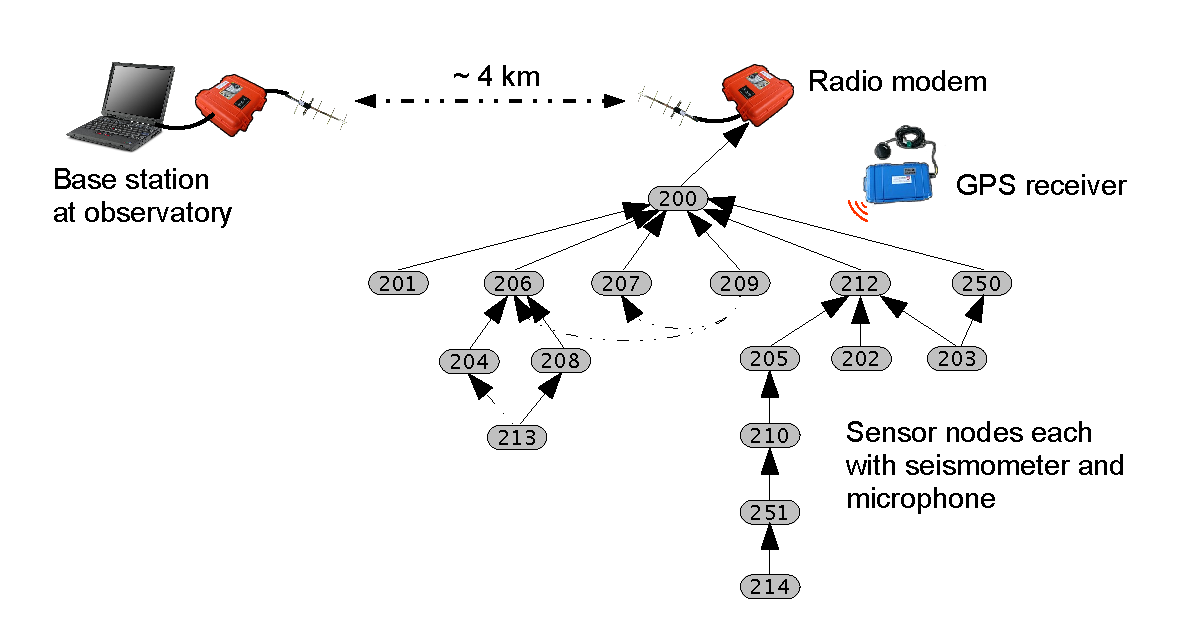
\includegraphics[width=1.0\hsize]{./3-evaluation/figs/schematic2.pdf}
\end{center}
\caption{\textbf{Sensor network architecture.} Nodes form a
multihop routing topology, relaying data via a long-distance radio
modem to the observatory. A GPS receiver is used to establish a global
timebase. The network topology shown here was used during
our deployment at Reventador.}
\end{figure}

\begin{figure}[t]
\label{evaluation-fig-map}
\begin{center}
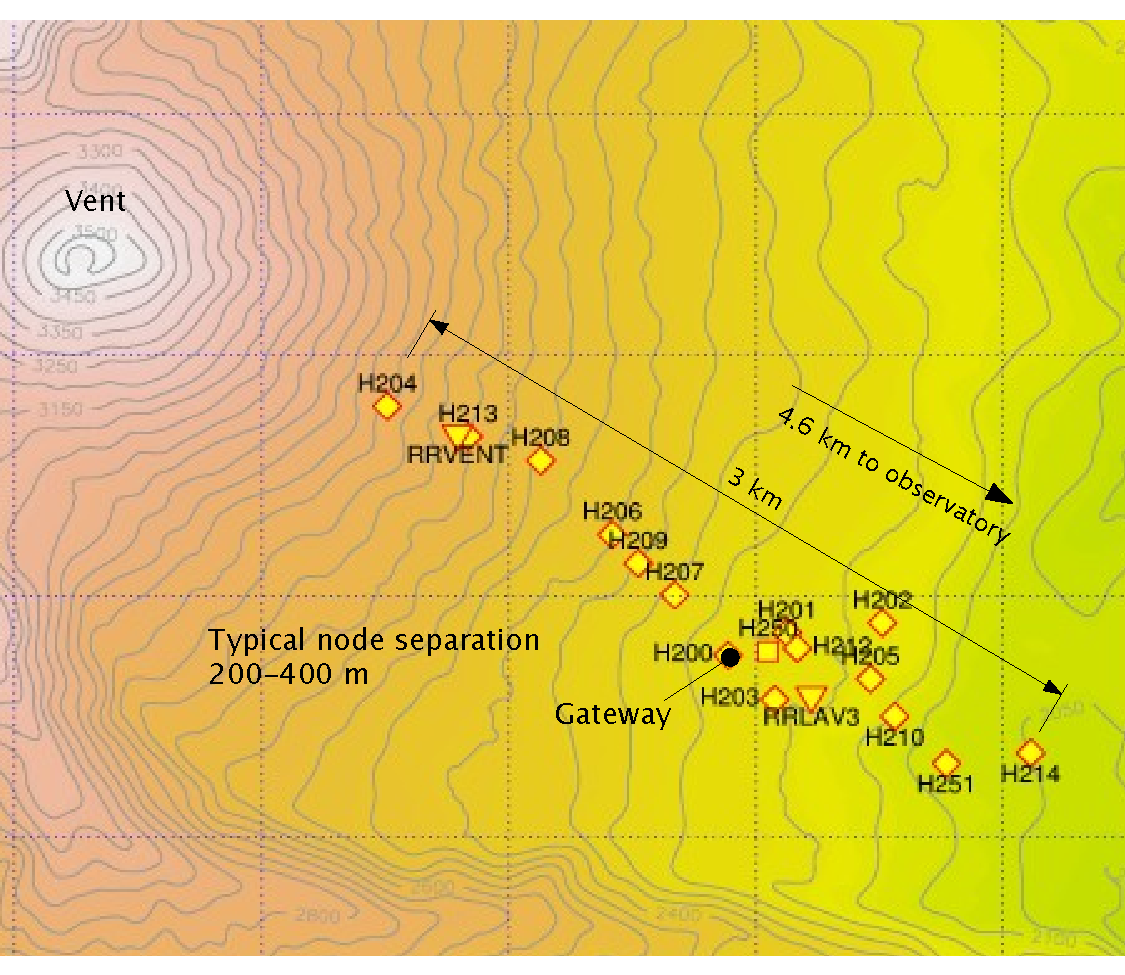
\includegraphics[width=1.0\hsize]{./3-evaluation/figs/reventador-map-crop.pdf}
\end{center}
\caption{\textbf{Map of sensor deployment at Volc\'{a}n Reventador.}
In addition to the 16~sensor nodes, two broadband seismometers
with data loggers (RRVENT and RRLAV3) were colocated with the network.}
\end{figure}

% MDW 26-Aug-06: I have revisited some of Jeff Johnson's suggestions
% in the below text; i.e., hyphenation on "broad-band" and so forth.

Our deployment at Reventador took place between August 1--19, 2005.
Reventador is an active volcano located in northern Ecuador, about 100~km
from Quito. 
%The volcano erupted with massive force in 2002, blanketing the streets of
%Quito with ash, closing schools and the airport. 
During this time, Reventador's activity consisted of small explosive events
that ejected ash and incandescent blocks several times a day. Associated
seismicity included numerous explosion earthquakes as well as
extended-duration shaking (tremor) and shallow rock-fracturing earthquakes.

We deployed 16~sensor nodes on the upper flanks of Reventador, as shown in
Figure~\ref{evaluation-fig-map}, over a 3~km linear configuration radiating
away from the vent. The resulting multihop topology is shown in
Figure~\ref{evaluation-fig-schematic}. The upper flanks of the volcano were
completely deforested by a large eruption in November 2002, allowing for
line-of-sight radio communication between adjacent sensor nodes.  Two
standalone seismic stations, consisting of a broadband sensor, a Reftek 130
data logger with 1~GByte flash memory cards, and a GPS receiver for
timestamping, were colocated with sensor nodes. The data from these stations
is essential to our network validation.
%described in
%Sections~\ref{evaluation-sec-eventdetection}~and~\ref{evaluation-sec-timing}.
The base station was located at a small hotel 4.6~km from the deployment
site.  The sensors were deployed for a total of 19~days, during which time
the network recorded data from 229~earthquakes, eruptions, and tremor events,
logging 107~MBytes of data. The long hike and lack of roads prevented
frequent returns to the deployment site, although we returned several times
to change batteries and perform other network maintenance.

%Colocated with our
%sensor network were two broadband seismometer stations,
%each using a Reftek~130 data logger with 1~GByte flash memory cards
%and a GPS receiver for timestamping. The data from these stations 
%is essential to our network validation, described in 
%Sections~\ref{sec-eventdetection}~and~\ref{sec-timing}.  
%The base station was located at 
%a small hotel 4.6~km from the deployment site. 

% MDW 26-Aug-06: I don't think this subsection is really needed. 
% Maybe the first paragraph could be added back somewhere; the rest is
% not pithy enough to warrant inclusion.

%\subsection{Design decisions}
%
%For this deployment our primary design goals were simplicity,
%statelessness, and robustness.  As such, we chose not to focus on
%aggressive power management, routing performance, fault tolerance
%(e.g. multiple base stations and GPS receivers), or scalability.  We
%plan to address these issues in future deployments.
%
%Some of our design decisions were influenced by the fact that the deployment
%site was a strenuous 3~hour hike from the observatory, meaning that we wanted
%to avoid problems that might require returning to the deployment
%site.  Other decisions were driven by more pragmatic reasons.  For example,
%although having a GPS receiver on each node would make the system more
%robust, we decided against it due to the increased cost, power, and
%deployment logistics.  Each GPS node requires a car battery to power it for a
%longer duration, making the deployment impractical given the difficult
%circumstances.  Instead we decided to equip only one node with a GPS receiver
%and use FTSP~\cite{ftsp} to synchronize the rest of the network.
%
%Finally, we point out that initially we planed on a 25~node network.
%However, because of various hardware failures we ended up with 16
%deployable nodes.

